\chapter{Analyser}
\label{cp:analyser}

La phase \textbf{Analyser} constitue le cœur de la démarche DMAIC. Après avoir défini le problème et mesuré les données pertinentes, il s'agit désormais d'identifier les causes profondes des non-conformités observées. Cette étape repose sur une investigation rigoureuse et structurée, mobilisant des outils statistiques et graphiques afin de distinguer les causes réelles des simples symptômes. L'objectif est de comprendre \textit{pourquoi} les écarts se produisent, avant toute tentative de correction ou d'amélioration.

Dans ce chapitre, nous mettons en œuvre plusieurs outils d'analyse causale appliqués aux données collectées sur le processus de fabrication étudié. Les résultats obtenus permettront d'orienter les actions d'amélioration présentées dans la phase suivante.

%------------------------------------------------------------------
\section{Analyse des causes racines des non-conformités}
\label{sec:analyse-causes-racines}

L'identification des causes racines est une étape essentielle pour garantir que les actions correctives menées s'attaquent aux origines réelles des défauts, et non à leurs manifestations superficielles. Plusieurs méthodes complémentaires sont employées à cet effet.

%------------------------------------------------------------------
\subsection{Diagramme ISHIKAWA}
\label{subsec:ishikawa}

Le diagramme d'Ishikawa, également appelé diagramme de cause-à-effet ou \textit{diagramme en arêtes de poisson}, est un outil visuel permettant de recenser et d'organiser l'ensemble des causes potentielles d'un effet indésirable. Développé par Kaoru Ishikawa dans les années 1960, il structure les causes selon les catégories classiques des \textbf{5M} : Matière, Milieu, Méthode, Machine et Main-d'œuvre.

Dans le contexte de notre étude, les catégories retenues ont été adaptées aux spécificités du processus de modélisation CATIA~V5. On distingue trois \textbf{causes techniques} --- Méthode, Géométrie et Logiciel --- et trois \textbf{causes opérationnelles} --- Utilisateur, Données~/~Fichier et Paramètres. L'effet ciblé regroupe les quatre types de défauts qualité identifiés sur les modèles CATIA~V5.

%--- Ishikawa colors (local) ---
\definecolor{ishitech}{HTML}{3D3B8E}
\definecolor{ishiops}{HTML}{0D6B53}
\definecolor{ishieff}{HTML}{6B1519}

\begin{figure}[htbp]
\centering
\vspace{1em}
\resizebox{\linewidth}{!}{%
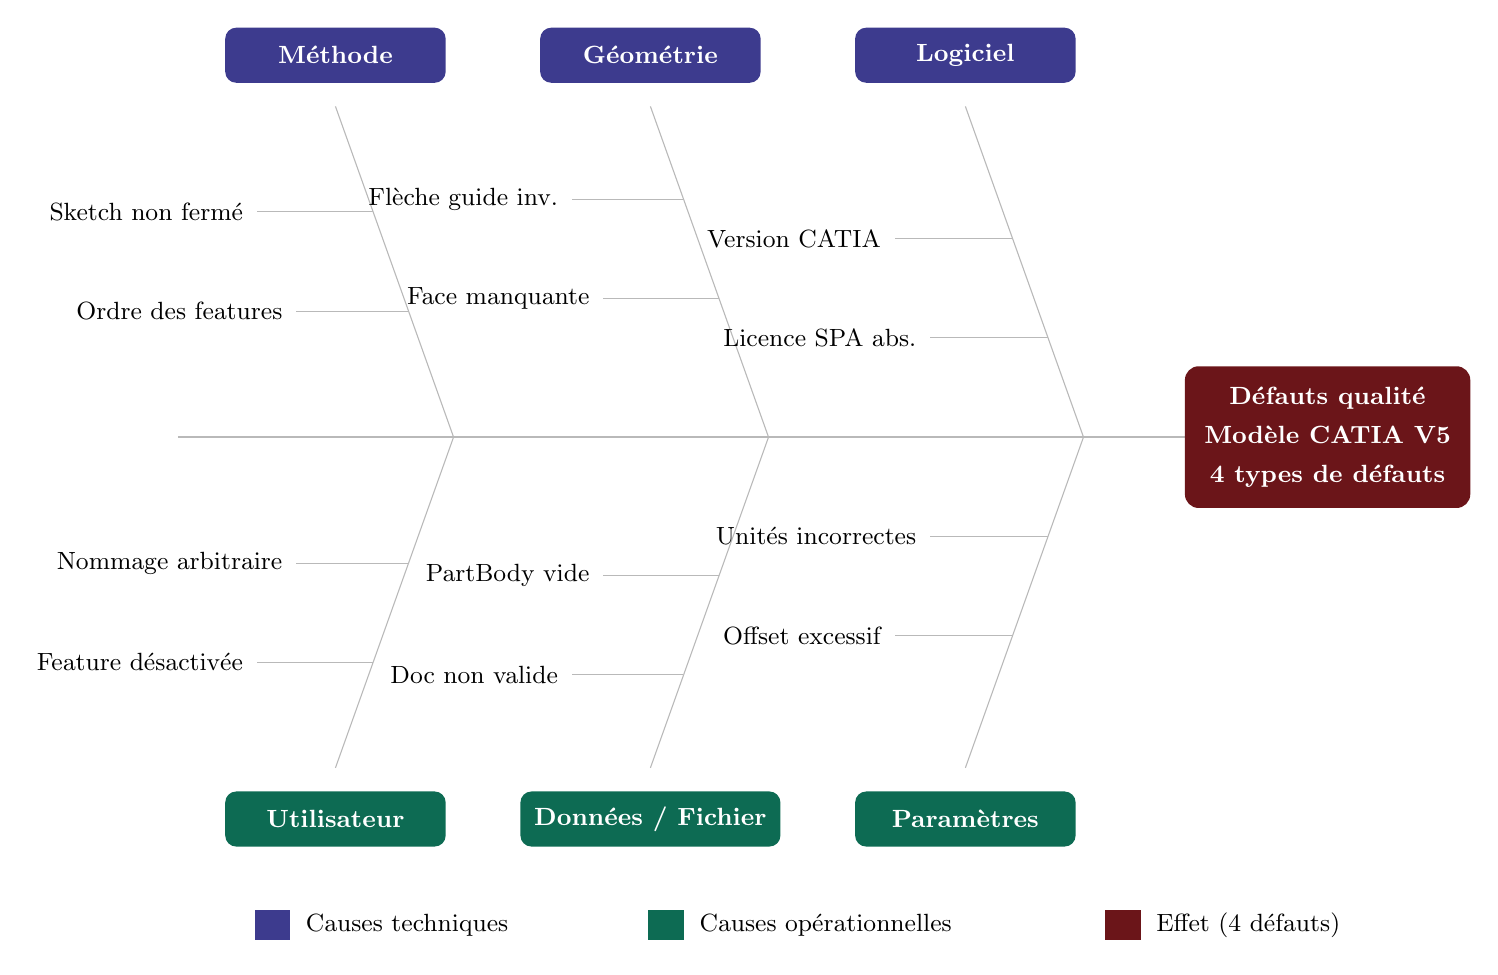
\begin{tikzpicture}[
    >=stealth,
    font=\small,
    % Styles
    techcat/.style={
        rectangle, rounded corners=4pt,
        fill=ishitech, text=white,
        font=\small\bfseries, align=center,
        inner sep=5pt, minimum width=2.8cm, minimum height=0.7cm
    },
    opscat/.style={
        rectangle, rounded corners=4pt,
        fill=ishiops, text=white,
        font=\small\bfseries, align=center,
        inner sep=5pt, minimum width=2.8cm, minimum height=0.7cm
    },
    effectbox/.style={
        rectangle, rounded corners=5pt,
        fill=ishieff, text=white,
        font=\small\bfseries, align=center,
        inner sep=7pt, minimum width=3cm, minimum height=1.8cm
    },
    bone/.style={draw=gray!55, thin},
    causelabel/.style={font=\small, text=black, align=center},
    legendsq/.style={rectangle, minimum width=0.45cm, minimum height=0.38cm, inner sep=0pt},
]


%--- Spine ---%
\draw[gray!55, thick, ->] (0,0) -- (13.0,0);

%--- Effect box ---%
\node[effectbox] at (14.6, 0) {Défauts qualité\\[3pt]Modèle CATIA V5\\[3pt]4 types de défauts};

%--- Main diagonal bones ---
% Spine intersect points: x = 3.5, 7.5, 11.5
% Category centre x:      2.0, 6.0, 10.0   (shifted ~1.5 left of intersect)
% Category centre y: +4.2 (top) / -4.2 (bottom)

% Top bones
\draw[bone] (2.0, 4.2) -- (3.5, 0);
\draw[bone] (6.0, 4.2) -- (7.5, 0);
\draw[bone] (10.0, 4.2) -- (11.5, 0);

% Bottom bones
\draw[bone] (2.0, -4.2) -- (3.5, 0);
\draw[bone] (6.0, -4.2) -- (7.5, 0);
\draw[bone] (10.0, -4.2) -- (11.5, 0);

%--- Category boxes ---
\node[techcat] at (2.0,  4.85) {Méthode};
\node[techcat] at (6.0,  4.85) {Géométrie};
\node[techcat] at (10.0, 4.85) {Logiciel};

\node[opscat] at (2.0,  -4.85) {Utilisateur};
\node[opscat] at (6.0,  -4.85) {Données / Fichier};
\node[opscat] at (10.0, -4.85) {Paramètres};

%--- Sub-causes ---
% Parametric helper: bone from (x0,y0) to (x1,0)
%   P(t) = (x0 + t*(x1-x0),  y0*(1-t))

% == Méthode: (2.0, 4.2) -> (3.5, 0), dx=1.5, dy=-4.2 ==
% t=0.32 -> (2.48,  2.86)
\draw[bone] (2.48,  2.86) -- (1.0,  2.86);
\node[causelabel, anchor=east] at (0.95, 2.86) {Sketch non fermé};
% t=0.62 -> (2.93,  1.60)
\draw[bone] (2.93,  1.60) -- (1.5,  1.60);
\node[causelabel, anchor=east] at (1.45, 1.60) {Ordre des features};

% == Géométrie: (6.0, 4.2) -> (7.5, 0) — stubs LEFT ==
% t=0.28 -> (6.42, 3.02)
\draw[bone] (6.42,  3.02) -- (5.0,  3.02);
\node[causelabel, anchor=east] at (4.95, 3.02) {Flèche guide inv.};
% t=0.58 -> (6.87, 1.76)
\draw[bone] (6.87,  1.76) -- (5.4,  1.76);
\node[causelabel, anchor=east] at (5.35, 1.76) {Face manquante};

% == Logiciel: (10.0, 4.2) -> (11.5, 0) — stubs LEFT ==
% t=0.40 -> (10.60, 2.52)
\draw[bone] (10.60, 2.52) -- (9.1,  2.52);
\node[causelabel, anchor=east] at (9.05, 2.52) {Version CATIA};
% t=0.70 -> (11.05, 1.26)
\draw[bone] (11.05, 1.26) -- (9.55, 1.26);
\node[causelabel, anchor=east] at (9.50, 1.26) {Licence SPA abs.};

% == Utilisateur: (2.0, -4.2) -> (3.5, 0) ==
% t=0.32 -> (2.48, -2.86)
\draw[bone] (2.48, -2.86) -- (1.0, -2.86);
\node[causelabel, anchor=east] at (0.95, -2.86) {Feature désactivée};
% t=0.62 -> (2.93, -1.60)
\draw[bone] (2.93, -1.60) -- (1.5, -1.60);
\node[causelabel, anchor=east] at (1.45, -1.60) {Nommage arbitraire};

% == Données/Fichier: (6.0, -4.2) -> (7.5, 0) — stubs LEFT ==
% t=0.28 -> (6.42, -3.02)
\draw[bone] (6.42, -3.02) -- (5.0, -3.02);
\node[causelabel, anchor=east] at (4.95, -3.02) {Doc non valide};
% t=0.58 -> (6.87, -1.76)
\draw[bone] (6.87, -1.76) -- (5.4, -1.76);
\node[causelabel, anchor=east] at (5.35, -1.76) {PartBody vide};

% == Paramètres: (10.0, -4.2) -> (11.5, 0) — stubs LEFT ==
% t=0.40 -> (10.60, -2.52)
\draw[bone] (10.60, -2.52) -- (9.1,  -2.52);
\node[causelabel, anchor=east] at (9.05, -2.52) {Offset excessif};
% t=0.70 -> (11.05, -1.26)
\draw[bone] (11.05, -1.26) -- (9.55, -1.26);
\node[causelabel, anchor=east] at (9.50, -1.26) {Unités incorrectes};

%--- Legend ---
\node[legendsq, fill=ishitech] at (1.2, -6.2) {};
\node[anchor=west, font=\small] at (1.5, -6.2) {Causes techniques};

\node[legendsq, fill=ishiops]  at (6.2, -6.2) {};
\node[anchor=west, font=\small] at (6.5, -6.2) {Causes opérationnelles};

\node[legendsq, fill=ishieff]  at (12.0, -6.2) {};
\node[anchor=west, font=\small] at (12.3, -6.2) {Effet (4 défauts)};

\end{tikzpicture}%
}
\caption{Diagramme d'Ishikawa --- causes racines des défauts qualité du modèle CATIA~V5.}
\label{fig:ishikawa}
\end{figure}

%==================================================================
\section{Arbres des causes par type de défaut}
\label{sec:arbres-causes}
%==================================================================

\subsection{Arbre des causes par défaut qualité}
\label{subsec:arbre-causes}

Afin d'approfondir l'analyse, un arbre des causes est construit pour chaque type de défaut identifié. Cette représentation hiérarchique permet de relier l'effet observé à ses causes directes, puis de descendre vers les causes racines sous-jacentes. Le premier défaut étudié est le volume nul (\textit{Part non solide}), détecté automatiquement par la macro VBS développée dans la phase Mesurer.

%--- Fault-tree colors (local) ---
\definecolor{fteffect}{HTML}{6B1519}
\definecolor{ftdirect}{HTML}{7B4A00}
\definecolor{ftroot}{HTML}{3D3D3D}

\begin{figure}[htbp]
\centering
\vspace{0.5em}
\resizebox{\linewidth}{!}{%
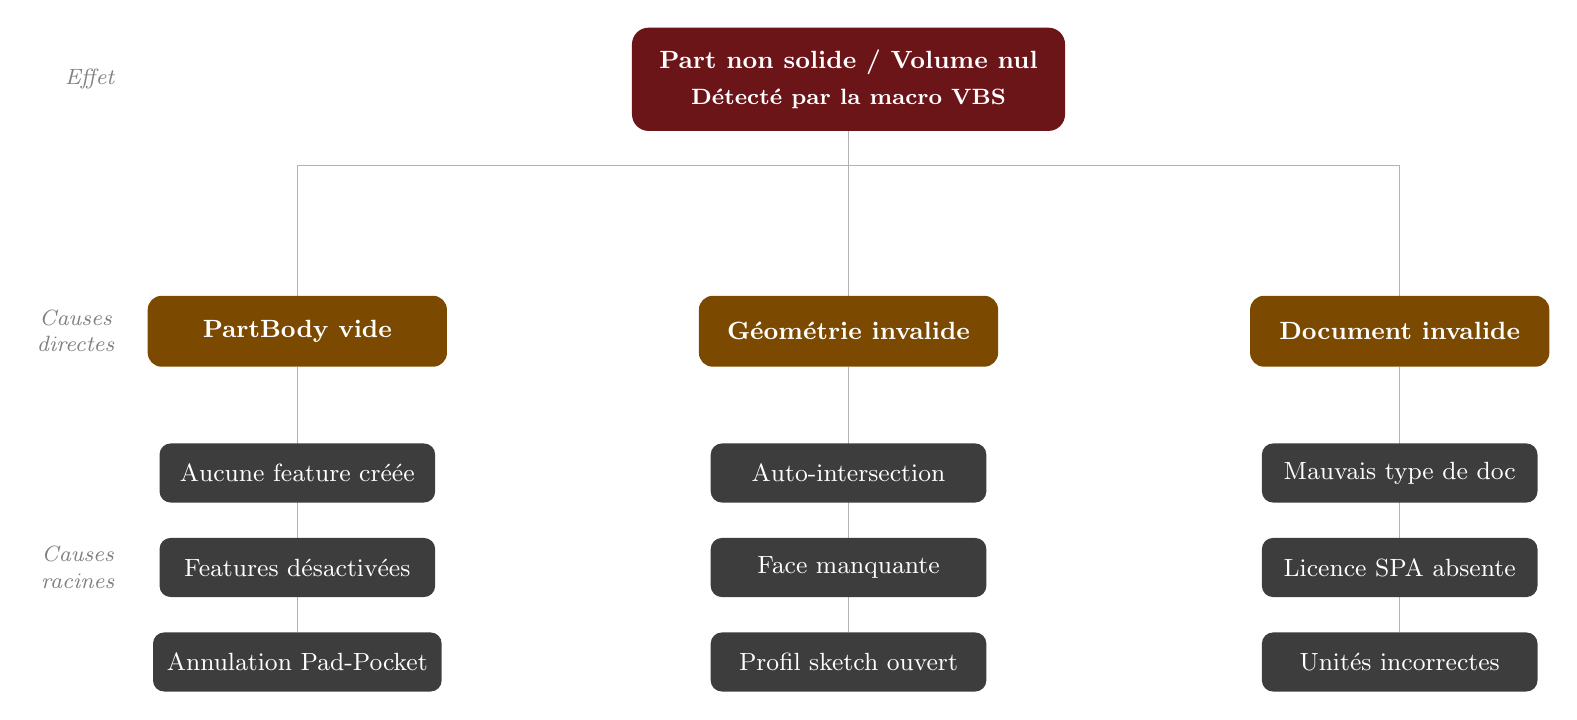
\begin{tikzpicture}[
    node distance=0pt,
    font=\small,
    effectnode/.style={
        rectangle, rounded corners=6pt,
        fill=fteffect, text=white,
        font=\small\bfseries, align=center,
        inner sep=8pt, minimum width=5.5cm, minimum height=1.1cm
    },
    directnode/.style={
        rectangle, rounded corners=5pt,
        fill=ftdirect, text=white,
        font=\small\bfseries, align=center,
        inner sep=6pt, minimum width=3.8cm, minimum height=0.9cm
    },
    rootnode/.style={
        rectangle, rounded corners=4pt,
        fill=ftroot, text=white,
        font=\small, align=center,
        inner sep=5pt, minimum width=3.5cm, minimum height=0.75cm
    },
    conn/.style={draw=gray!60, thin},
]

% ============================================================
% Draw ALL lines first — nodes are painted on top afterwards
% Node geometry (minimum heights in cm = abstract units here):
%   effectnode h=1.1  → south at y = -0.55
%   directnode h=0.9  → south at y_center - 0.45
%   rootnode   h=0.75 → north at y_center + 0.375, south at y_center - 0.375
%
%   d1/d2/d3 at y=-3.2  → south = -3.65
%   r*a at y=-5.0  → north=-4.625, south=-5.375
%   r*b at y=-6.2  → north=-5.825, south=-6.575
%   r*c at y=-7.4  → north=-7.025
% ============================================================

% Effect -> horizontal bus
\draw[conn] (9, -0.55) -- (9, -1.1);
\draw[conn] (2, -1.1) -- (16, -1.1);

% Bus -> top of each direct-cause box
\draw[conn] (2,  -1.1) -- (2,  -2.75);
\draw[conn] (9,  -1.1) -- (9,  -2.75);
\draw[conn] (16, -1.1) -- (16, -2.75);

% Vertical trunks: direct-cause bottom -> below last root
\draw[conn] (2,  -3.65) -- (2,  -7.025);
\draw[conn] (9,  -3.65) -- (9,  -7.025);
\draw[conn] (16, -3.65) -- (16, -7.025);

% ============================================================
% Now draw all nodes ON TOP of the lines
% ============================================================

%--- Effect ---
\node[effectnode] at (9, 0) {Part non solide / Volume nul\\[2pt]{\footnotesize Détecté par la macro VBS}};

%--- Direct causes ---
\node[directnode] at (2,  -3.2) {PartBody vide};
\node[directnode] at (9,  -3.2) {Géométrie invalide};
\node[directnode] at (16, -3.2) {Document invalide};

%--- Root causes – PartBody vide ---
\node[rootnode] at (2, -5.0) {Aucune feature créée};
\node[rootnode] at (2, -6.2) {Features désactivées};
\node[rootnode] at (2, -7.4) {Annulation Pad-Pocket};

%--- Root causes – Géométrie invalide ---
\node[rootnode] at (9, -5.0) {Auto-intersection};
\node[rootnode] at (9, -6.2) {Face manquante};
\node[rootnode] at (9, -7.4) {Profil sketch ouvert};

%--- Root causes – Document invalide ---
\node[rootnode] at (16, -5.0) {Mauvais type de doc};
\node[rootnode] at (16, -6.2) {Licence SPA absente};
\node[rootnode] at (16, -7.4) {Unités incorrectes};

%--- Side labels ---
\node[font=\footnotesize\itshape, text=gray, anchor=east, align=center] at (-0.2,  0)    {Effet};
\node[font=\footnotesize\itshape, text=gray, anchor=east, align=center] at (-0.2, -3.2)  {Causes\\directes};
\node[font=\footnotesize\itshape, text=gray, anchor=east, align=center] at (-0.2, -6.2)  {Causes\\racines};

\end{tikzpicture}%
}
\caption{Arbre des causes --- défaut \textit{Part non solide / Volume nul}.}
\label{fig:arbre-causes-volume-nul}
\end{figure}

%------------------------------------------------------------------
\subsection{Surface auto-intersectante}
\label{subsec:arbre-auto-intersection}

Le deuxième défaut analysé est la \textbf{surface auto-intersectante}, caractéristique des défauts géométriques détectés dans le module GSD (Generative Shape Design) de CATIA~V5. Ce type de défaut survient lorsque la surface générée se recoupe elle-même, rendant la géométrie inexploitable pour les opérations aval. L'arbre des causes ci-dessous identifie trois familles de causes directes : le profil source, l'opération de surface et les paramètres de construction.

\definecolor{fteff2}{HTML}{6B1519}
\definecolor{ftdir2}{HTML}{7B4A00}

\begin{figure}[htbp]
\centering
\vspace{0.5em}
\resizebox{\linewidth}{!}{%
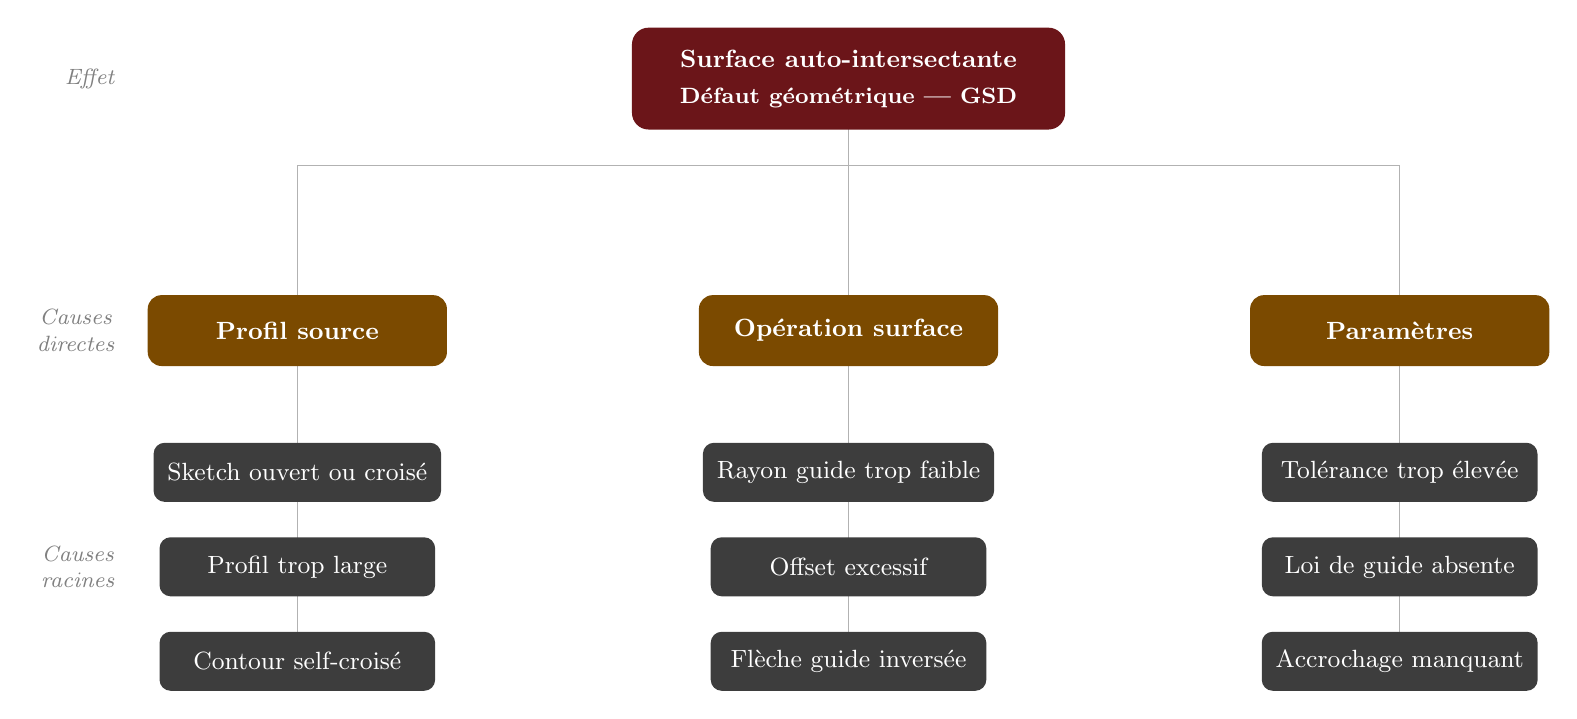
\begin{tikzpicture}[
    font=\small,
    effectnode/.style={rectangle, rounded corners=6pt, fill=fteff2, text=white,
        font=\small\bfseries, align=center, inner sep=8pt,
        minimum width=5.5cm, minimum height=1.1cm},
    directnode/.style={rectangle, rounded corners=5pt, fill=ftdir2, text=white,
        font=\small\bfseries, align=center, inner sep=6pt,
        minimum width=3.8cm, minimum height=0.9cm},
    rootnode/.style={rectangle, rounded corners=4pt, fill=ftroot, text=white,
        font=\small, align=center, inner sep=5pt,
        minimum width=3.5cm, minimum height=0.75cm},
    conn/.style={draw=gray!60, thin},
]
% --- Lines first ---
\draw[conn] (9,-0.55) -- (9,-1.1);
\draw[conn] (2,-1.1) -- (16,-1.1);
\draw[conn] (2,-1.1)  -- (2,-2.75);
\draw[conn] (9,-1.1)  -- (9,-2.75);
\draw[conn] (16,-1.1) -- (16,-2.75);
\draw[conn] (2,-3.65)  -- (2,-7.025);
\draw[conn] (9,-3.65)  -- (9,-7.025);
\draw[conn] (16,-3.65) -- (16,-7.025);
% --- Nodes ---
\node[effectnode] at (9,0) {Surface auto-intersectante\\[2pt]{\footnotesize Défaut géométrique --- GSD}};
\node[directnode] at (2,-3.2)  {Profil source};
\node[directnode] at (9,-3.2)  {Opération surface};
\node[directnode] at (16,-3.2) {Paramètres};
\node[rootnode] at (2,-5.0)  {Sketch ouvert ou croisé};
\node[rootnode] at (2,-6.2)  {Profil trop large};
\node[rootnode] at (2,-7.4)  {Contour self-croisé};
\node[rootnode] at (9,-5.0)  {Rayon guide trop faible};
\node[rootnode] at (9,-6.2)  {Offset excessif};
\node[rootnode] at (9,-7.4)  {Flèche guide inversée};
\node[rootnode] at (16,-5.0) {Tolérance trop élevée};
\node[rootnode] at (16,-6.2) {Loi de guide absente};
\node[rootnode] at (16,-7.4) {Accrochage manquant};
% --- Side labels ---
\node[font=\footnotesize\itshape, text=gray, anchor=east, align=center] at (-0.2,0)    {Effet};
\node[font=\footnotesize\itshape, text=gray, anchor=east, align=center] at (-0.2,-3.2) {Causes\\directes};
\node[font=\footnotesize\itshape, text=gray, anchor=east, align=center] at (-0.2,-6.2) {Causes\\racines};
\end{tikzpicture}%
}
\caption{Arbre des causes --- défaut \textit{Surface auto-intersectante}.}
\label{fig:arbre-causes-auto-intersection}
\end{figure}

%------------------------------------------------------------------
\subsection{Surface vrillée}
\label{subsec:arbre-surface-vrillee}

La \textbf{surface vrillée} (\textit{twisted}) constitue le troisième défaut étudié. Il s'agit d'un défaut d'orientation propre aux opérations Sweep et Loft du module GSD : la surface se tord le long de la trajectoire guide, produisant une géométrie incorrecte. Les causes sont regroupées en trois catégories — orientation des courbes, géométrie du guide, et paramétrage de l'opération.

\definecolor{fteff3}{HTML}{5C3A00}
\definecolor{ftdir3}{HTML}{1F3E6E}

\begin{figure}[htbp]
\centering
\vspace{0.5em}
\resizebox{\linewidth}{!}{%
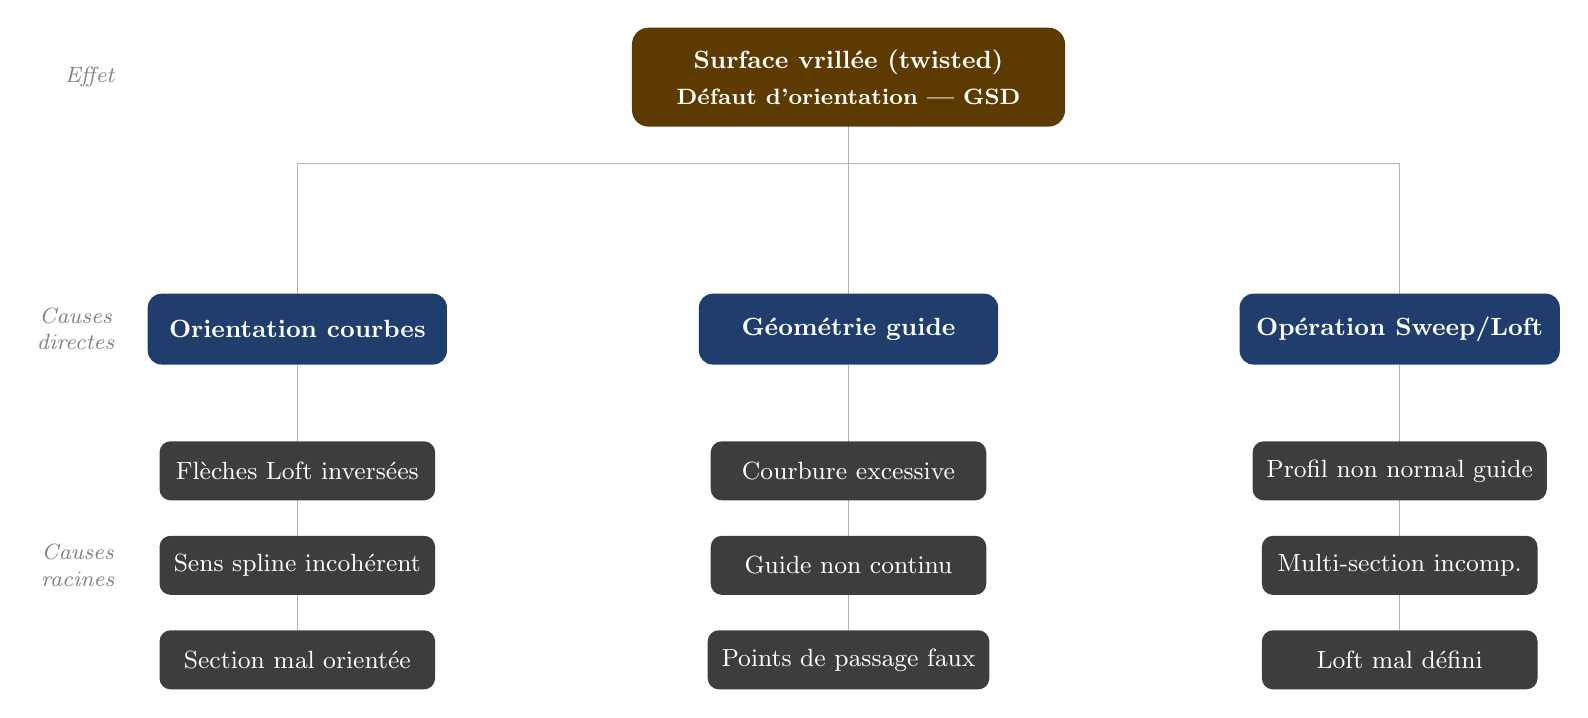
\begin{tikzpicture}[
    font=\small,
    effectnode/.style={rectangle, rounded corners=6pt, fill=fteff3, text=white,
        font=\small\bfseries, align=center, inner sep=8pt,
        minimum width=5.5cm, minimum height=1.1cm},
    directnode/.style={rectangle, rounded corners=5pt, fill=ftdir3, text=white,
        font=\small\bfseries, align=center, inner sep=6pt,
        minimum width=3.8cm, minimum height=0.9cm},
    rootnode/.style={rectangle, rounded corners=4pt, fill=ftroot, text=white,
        font=\small, align=center, inner sep=5pt,
        minimum width=3.5cm, minimum height=0.75cm},
    conn/.style={draw=gray!60, thin},
]
% --- Lines first ---
\draw[conn] (9,-0.55) -- (9,-1.1);
\draw[conn] (2,-1.1) -- (16,-1.1);
\draw[conn] (2,-1.1)  -- (2,-2.75);
\draw[conn] (9,-1.1)  -- (9,-2.75);
\draw[conn] (16,-1.1) -- (16,-2.75);
\draw[conn] (2,-3.65)  -- (2,-7.025);
\draw[conn] (9,-3.65)  -- (9,-7.025);
\draw[conn] (16,-3.65) -- (16,-7.025);
% --- Nodes ---
\node[effectnode] at (9,0) {Surface vrillée (twisted)\\[2pt]{\footnotesize Défaut d'orientation --- GSD}};
\node[directnode] at (2,-3.2)  {Orientation courbes};
\node[directnode] at (9,-3.2)  {Géométrie guide};
\node[directnode] at (16,-3.2) {Opération Sweep/Loft};
\node[rootnode] at (2,-5.0)  {Flèches Loft inversées};
\node[rootnode] at (2,-6.2)  {Sens spline incohérent};
\node[rootnode] at (2,-7.4)  {Section mal orientée};
\node[rootnode] at (9,-5.0)  {Courbure excessive};
\node[rootnode] at (9,-6.2)  {Guide non continu};
\node[rootnode] at (9,-7.4)  {Points de passage faux};
\node[rootnode] at (16,-5.0) {Profil non normal guide};
\node[rootnode] at (16,-6.2) {Multi-section incomp.};
\node[rootnode] at (16,-7.4) {Loft mal défini};
% --- Side labels ---
\node[font=\footnotesize\itshape, text=gray, anchor=east, align=center] at (-0.2,0)    {Effet};
\node[font=\footnotesize\itshape, text=gray, anchor=east, align=center] at (-0.2,-3.2) {Causes\\directes};
\node[font=\footnotesize\itshape, text=gray, anchor=east, align=center] at (-0.2,-6.2) {Causes\\racines};
\end{tikzpicture}%
}
\caption{Arbre des causes --- défaut \textit{Surface vrillée}.}
\label{fig:arbre-causes-surface-vrillee}
\end{figure}

%------------------------------------------------------------------
\subsection{Non-conformité de nommage}
\label{subsec:arbre-nommage}

Le quatrième et dernier défaut traité concerne la \textbf{non-conformité de nommage} des données CATIA~V5. Bien qu'il n'entraîne pas de défaillance géométrique immédiate, un nommage arbitraire ou incohérent compromet la traçabilité, la maintenabilité et l'automatisation des traitements. Les causes sont articulées autour du nommage des features, des fichiers et des paramètres.

\definecolor{fteff4}{HTML}{3D3B8E}
\definecolor{ftdir4}{HTML}{0D5C47}

\begin{figure}[htbp]
\centering
\vspace{0.5em}
\resizebox{\linewidth}{!}{%
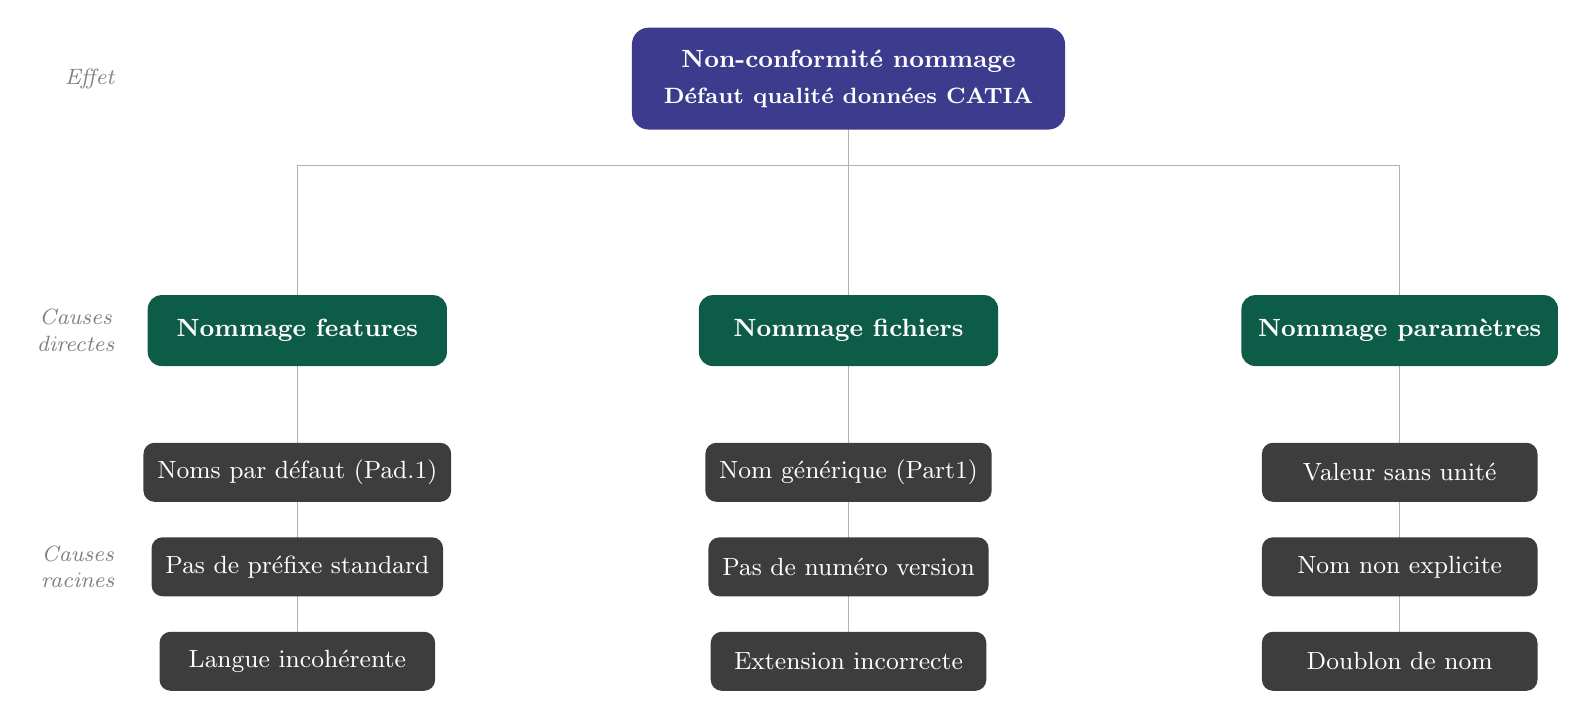
\begin{tikzpicture}[
    font=\small,
    effectnode/.style={rectangle, rounded corners=6pt, fill=fteff4, text=white,
        font=\small\bfseries, align=center, inner sep=8pt,
        minimum width=5.5cm, minimum height=1.1cm},
    directnode/.style={rectangle, rounded corners=5pt, fill=ftdir4, text=white,
        font=\small\bfseries, align=center, inner sep=6pt,
        minimum width=3.8cm, minimum height=0.9cm},
    rootnode/.style={rectangle, rounded corners=4pt, fill=ftroot, text=white,
        font=\small, align=center, inner sep=5pt,
        minimum width=3.5cm, minimum height=0.75cm},
    conn/.style={draw=gray!60, thin},
]
% --- Lines first ---
\draw[conn] (9,-0.55) -- (9,-1.1);
\draw[conn] (2,-1.1) -- (16,-1.1);
\draw[conn] (2,-1.1)  -- (2,-2.75);
\draw[conn] (9,-1.1)  -- (9,-2.75);
\draw[conn] (16,-1.1) -- (16,-2.75);
\draw[conn] (2,-3.65)  -- (2,-7.025);
\draw[conn] (9,-3.65)  -- (9,-7.025);
\draw[conn] (16,-3.65) -- (16,-7.025);
% --- Nodes ---
\node[effectnode] at (9,0) {Non-conformité nommage\\[2pt]{\footnotesize Défaut qualité données CATIA}};
\node[directnode] at (2,-3.2)  {Nommage features};
\node[directnode] at (9,-3.2)  {Nommage fichiers};
\node[directnode] at (16,-3.2) {Nommage paramètres};
\node[rootnode] at (2,-5.0)  {Noms par défaut (Pad.1)};
\node[rootnode] at (2,-6.2)  {Pas de préfixe standard};
\node[rootnode] at (2,-7.4)  {Langue incohérente};
\node[rootnode] at (9,-5.0)  {Nom générique (Part1)};
\node[rootnode] at (9,-6.2)  {Pas de numéro version};
\node[rootnode] at (9,-7.4)  {Extension incorrecte};
\node[rootnode] at (16,-5.0) {Valeur sans unité};
\node[rootnode] at (16,-6.2) {Nom non explicite};
\node[rootnode] at (16,-7.4) {Doublon de nom};
% --- Side labels ---
\node[font=\footnotesize\itshape, text=gray, anchor=east, align=center] at (-0.2,0)    {Effet};
\node[font=\footnotesize\itshape, text=gray, anchor=east, align=center] at (-0.2,-3.2) {Causes\\directes};
\node[font=\footnotesize\itshape, text=gray, anchor=east, align=center] at (-0.2,-6.2) {Causes\\racines};
\end{tikzpicture}%
}
\caption{Arbre des causes --- défaut \textit{Non-conformité de nommage}.}
\label{fig:arbre-causes-nommage}
\end{figure}

%==================================================================
\section{Convention de nommage}
\label{sec:naming-macro}
%==================================================================

%------------------------------------------------------------------
\subsection{Déroulement global de la macro}
\label{subsec:nm-deroulement}

% TODO : contenu à remplir --- texte descriptif et organigrammes à insérer ici.

%==================================================================
\section{Compréhension de la macro \texttt{silver\_faces.vbs}}
\label{sec:silver-faces-macro}
%==================================================================

%------------------------------------------------------------------
\subsection{Paramètres de configuration de la macro}
\label{subsec:sf-constantes}

La macro repose sur trois constantes dont les valeurs pilotent l'ensemble de la logique de détection et de correction :

\begin{table}[htbp]
\centering
\caption{Constantes de configuration de \texttt{silver\_faces.vbs}.}
\label{tab:sf-constantes}
\begin{tabularx}{\textwidth}{llX}
\toprule
\textbf{Constante} & \textbf{Valeur} & \textbf{Signification} \\
\midrule
SEUIL\_MM2    & \(0{,}01\ \text{mm}^2\)   & Toute surface dont l'aire est inférieure à ce seuil est considérée comme une silver face. \\
SEUIL\_DELETE & \(0{,}0001\ \text{mm}^2\) & En dessous de cette valeur, la surface est quasi-nulle et peut être supprimée directement. \\
HEALING\_DIST & \(0{,}1\ \text{mm}\)       & Distance de fusion utilisée lors de l'opération de Healing : les surfaces distantes de moins de \(0{,}1\ \text{mm}\) sont fusionnées. \\
\bottomrule
\end{tabularx}
\end{table}

%------------------------------------------------------------------
\subsection{Déroulement global de la macro}
\label{subsec:sf-deroulement}

La macro est décomposée en trois étapes principales, décrites ci-après.

\subsubsection{Étape 1: \texttt{CATMain()}}
\label{subsubsec:sf-catmain}

\begin{enumerate}
    \item[•] récupère le \textbf{document actif} dans CATIA.
    \item[•] vérifie son \textbf{type} :
        \begin{itemize}
            \item[•] Part seul (\texttt{.CATPart})
            \item[•] Product (\texttt{.CATProduct})
        \end{itemize}
    \item[•] appelle \texttt{ScanPart} pour détecter les silver faces.
    \item[•] affiche un \textbf{rapport} indiquant le nombre total de surfaces vérifiées, le nombre de silver faces trouvées, leurs noms, emplacements, aires et la stratégie de réparation applicable.
    \item[•] demande une \textbf{confirmation} à l'utilisateur avant d'appliquer les corrections.
    \item[•] si l'utilisateur confirme, la Macro appelle \texttt{CorrigerPart} pour effectuer les corrections.
\end{enumerate}

\begin{figure}[htbp]
    \centering
    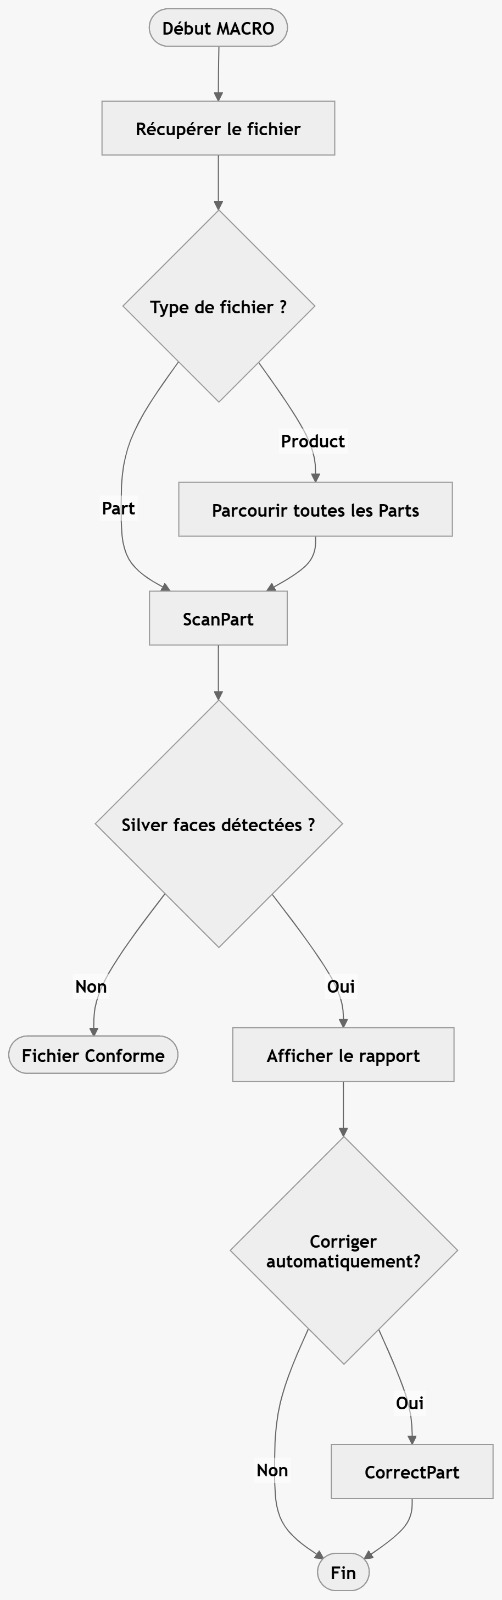
\includegraphics[height=0.85\textheight,keepaspectratio]{image/SILVER-FACE/CatMain_Silver_Face_TD.jpeg}
    \caption{Organigramme de la fonction \texttt{CATMain()} --- vue globale de la macro.}
    \label{fig:sf-flowchart-catmain}
\end{figure}

\subsubsection{Étape 2: \texttt{ScanPart()}}
\label{subsubsec:sf-scanpart}

Cette fonction inspecte l'ensemble des surfaces du Part et mesure leur aire.

La mesure utilise le \textbf{SPAWorkbench} de CATIA via l'objet \texttt{Measurable}. La propriété \texttt{.Area} est retournée en $\text{m}^2$ puis convertie en $\text{mm}^2$ (× 1\,000\,000).

Pour chaque silver face détectée, sont enregistrés : son nom, le Part et le dossier la contenant, son aire exacte en $\text{mm}^2$, et la stratégie de réparation associée :
\begin{itemize}
    \item[•] \textbf{Suppression}: si (l'aire $< 0{,}0001\ \text{mm}^2$).
    \item[•] \textbf{Healing}: si 
    ($0{,}0001 \leq \text{aire} < 0{,}01\ \text{mm}^2$).
\end{itemize}

\begin{figure}[htbp]
    \centering
    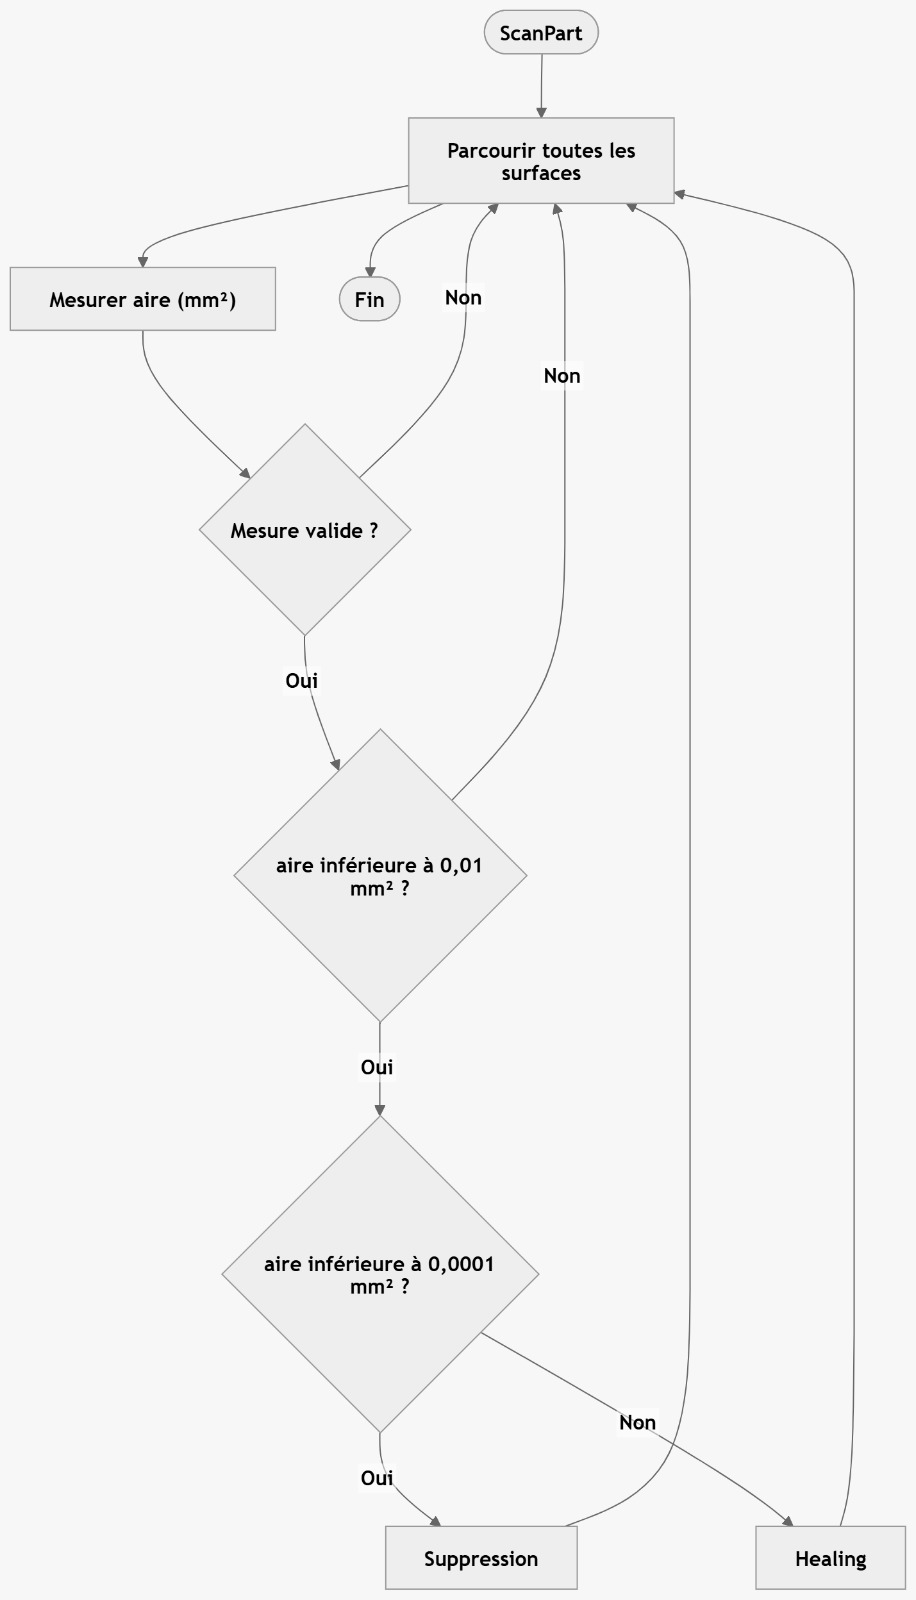
\includegraphics[height=0.85\textheight,keepaspectratio]{image/SILVER-FACE/ScanPart_Silver_Face_TD.jpeg}
    \caption{Organigramme de la fonction \texttt{ScanPart()} --- détection des silver faces.}
    \label{fig:sf-flowchart-scanpart}
\end{figure}

\subsubsection{Étape 3: \texttt{CorrigerPart()}}
\label{subsubsec:sf-corriger}

Cette fonction applique deux stratégies de correction automatique.

\paragraph{Suppression directe}
Appliquée lorsque l'aire est inférieure à $0{,}0001\ \text{mm}^2$. La surface est sélectionnée via \texttt{Selection.Add} puis supprimée par \texttt{Selection.Delete}, reproduisant l'action manuelle d'un utilisateur qui sélectionne et efface l'élément. La boucle se déroule \textbf{en sens inverse} pour éviter la désynchronisation des indices lors des suppressions successives.

\paragraph{Healing}
Le \textbf{Healing} est un outil de réparation CATIA qui:
\begin{enumerate}
    \item[•] prend un ensemble de surfaces ;
    \item[•] détecte les micro-écarts ou chevauchements entre elles ;
    \item[•] comble ou ferme ces écarts dans la tolérance \texttt{HEALING\_DIST} = $0{,}1\ \text{mm}$ ;
    \item[•] produit un groupe de surfaces « guéri » exempt de silver faces.
\end{enumerate}

\begin{figure}[htbp]
    \centering
    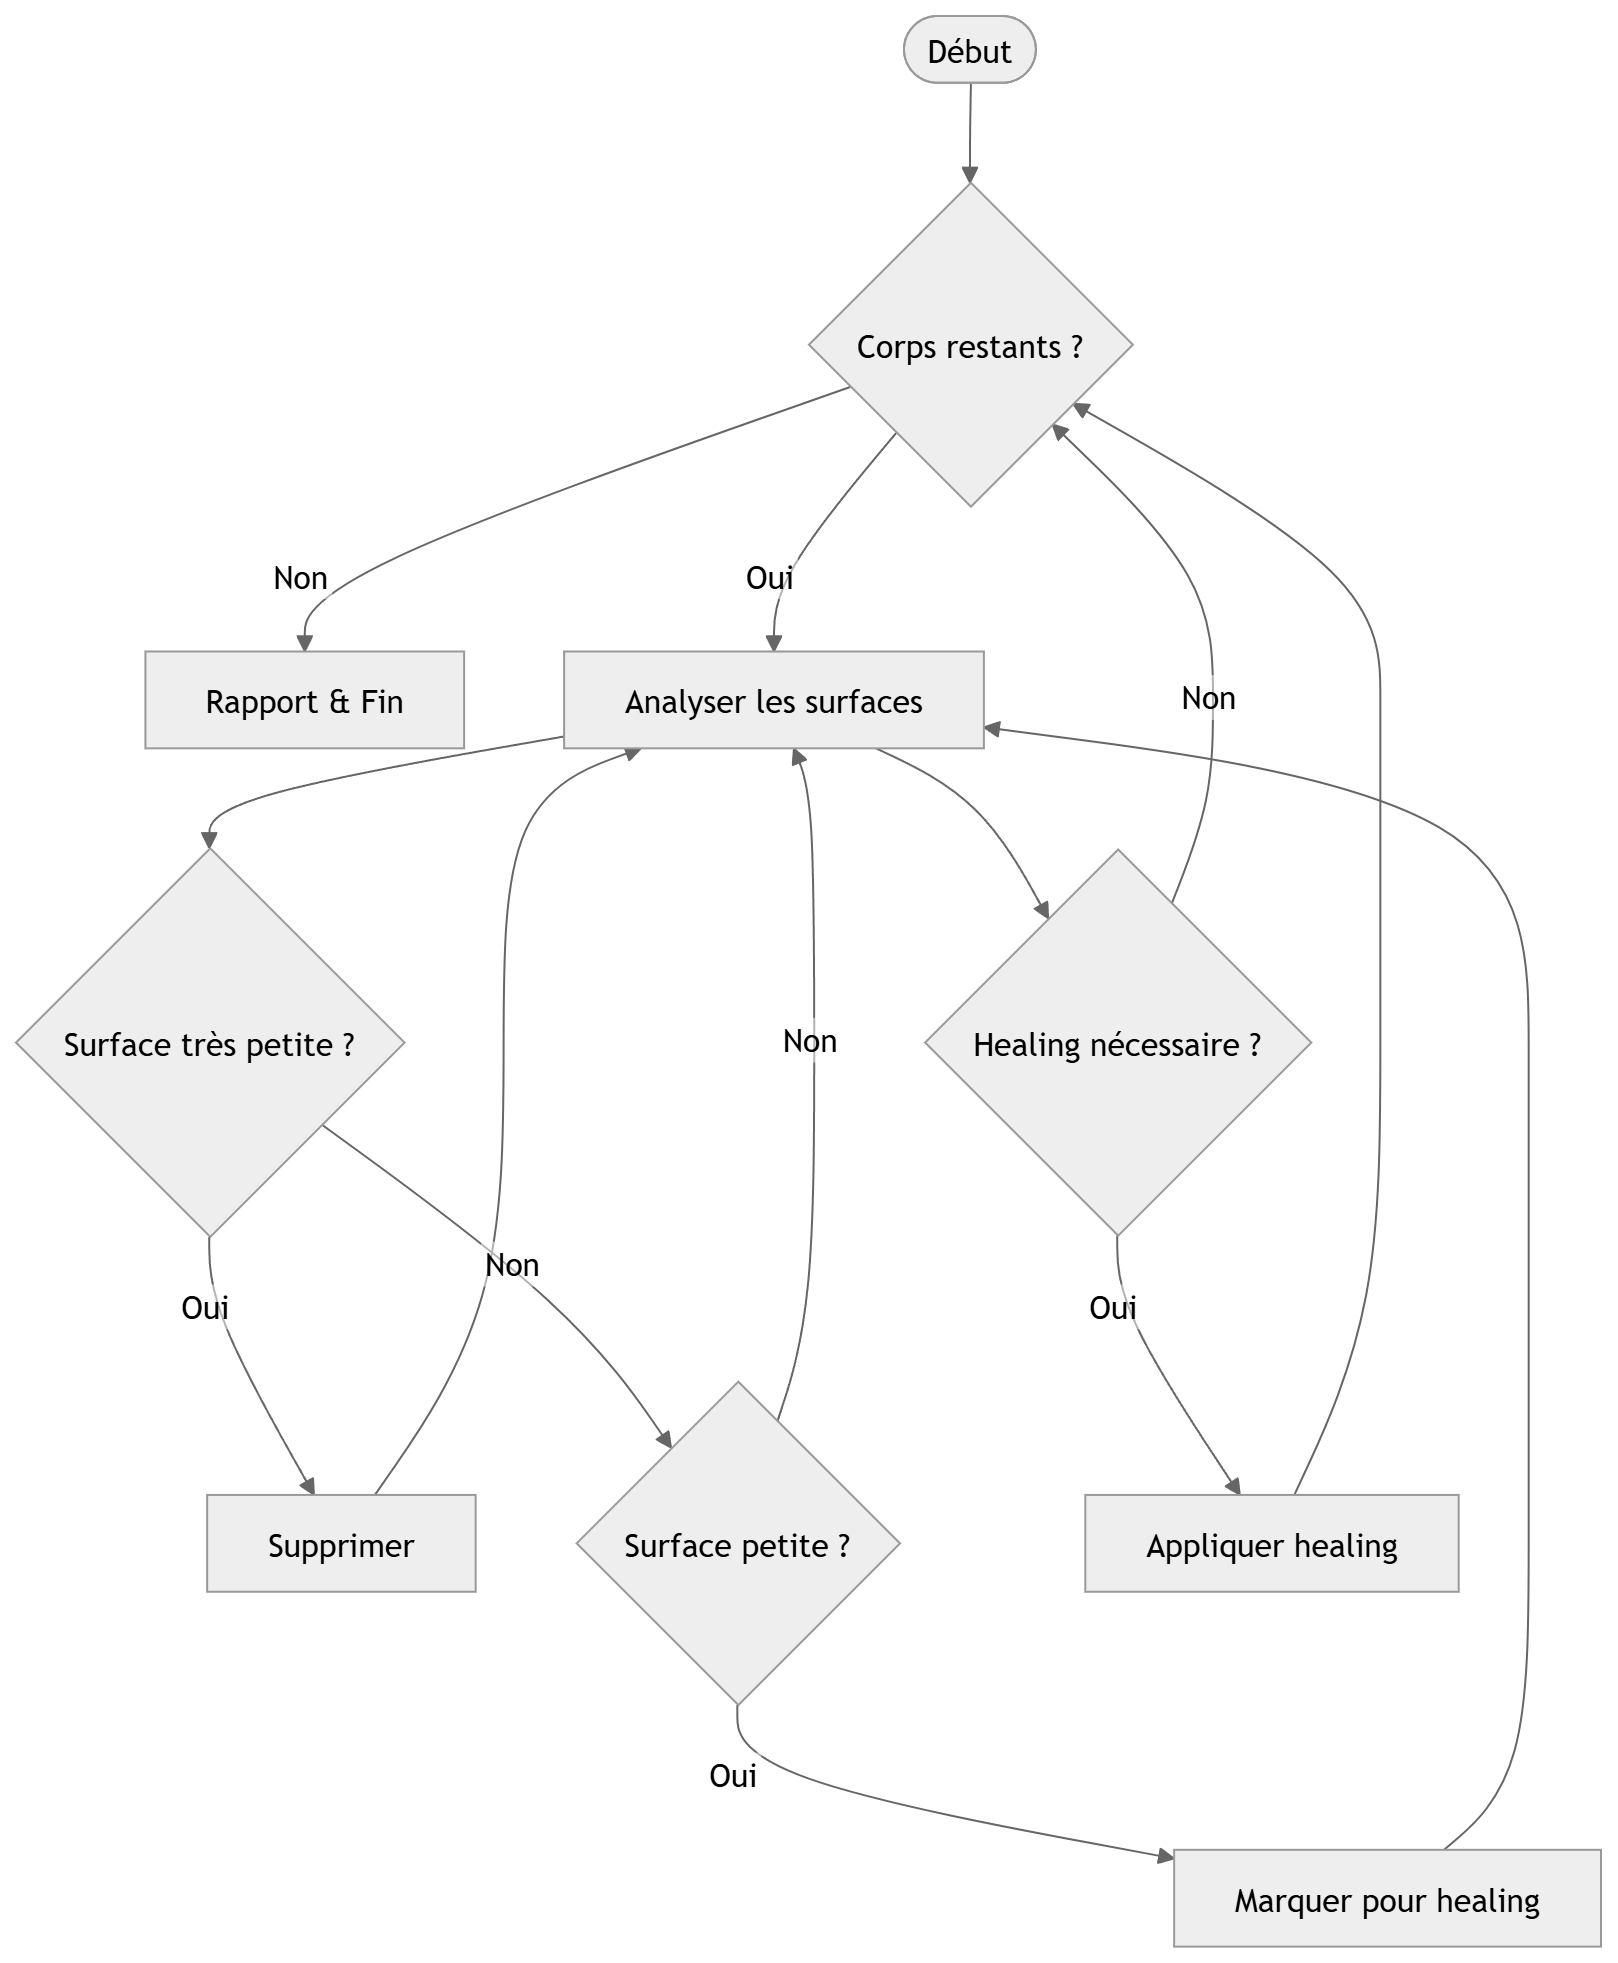
\includegraphics[height=0.85\textheight,keepaspectratio]{image/SILVER-FACE/Corriger_silver_face_TD.png}
    \caption{Organigramme de la fonction \texttt{CorrigerPart()} --- stratégies de correction.}
    \label{fig:sf-flowchart-corriger}
\end{figure}